% arara: pdflatex: { shell: on }
% arara: biber
% arara: pdflatex
% arara: pdflatex
% --------------------------------------------------------------------------
% the TRANSLATIONS package
% 
%   a simple translator
% 
% --------------------------------------------------------------------------
% Clemens Niederberger
% Web:    https://github.com/cgnieder/translations/
% E-Mail: contact@mychemistry.eu
% --------------------------------------------------------------------------
% Copyright 2011-2014 Clemens Niederberger
% 
% This work may be distributed and/or modified under the
% conditions of the LaTeX Project Public License, either version 1.3
% of this license or (at your option) any later version.
% The latest version of this license is in
%   http://www.latex-project.org/lppl.txt
% and version 1.3 or later is part of all distributions of LaTeX
% version 2005/12/01 or later.
% 
% This work has the LPPL maintenance status `maintained'.
% 
% The Current Maintainer of this work is Clemens Niederberger.
% --------------------------------------------------------------------------
% The translations package is part of the exsheets bundle
% --------------------------------------------------------------------------
% If you have any ideas, questions, suggestions or bugs to report, please
% feel free to contact me.
% --------------------------------------------------------------------------
\documentclass[load-preamble+,babel-options={french,spanish,ngerman,english}]{cnltx-doc}
% ----------------------------------------------------------------------------
% document layout and typographic features
\setcnltx{
  package  = {translations} ,
  authors  = Clemens Niederberger ,
  email    = contact@mychemistry.eu ,
  url      = https://github.com/cgnieder/translations/ ,
  info     = {Internationalization of \LaTeXe\ Packages} ,
  add-cmds = {
    baselanguage,
    DeclareDictTranslation,
    DeclareLanguage,
    DeclareLanguageAlias,
    DeclareLanguageDialect,
    DeclareTranslation,
    DeclareTranslationFallback,
    GetTranslation,
    GetTranslationFor,
    LoadDictionary,
    LoadDictionaryFor,
    NewTranslation,
    ProvideDictionaryFor,
    ProvideDictTranslation,
    RenewTranslation,
    SaveTranslation,
    SaveTranslationFor
  } ,
  add-silent-cmds = {
    cuisine,kitchen,mypackage@title
  } ,
  makeindex-setup = {options={-s cnltx.ist},columns=3,columnsep=1em} ,
  index-setup = {othercode=\footnotesize,level=\addsec,noclearpage}
}

\microtypesetup{tracking=scshape}

\defbibheading{bibliography}[\bibname]{\addsec{#1}}

\usepackage{csquotes}

\usepackage{embrac}[2012/06/29]
  \ChangeEmph{[}[,.02em]{]}[.055em,-.08em]
  \ChangeEmph{(}[-.01em,.04em]{)}[.04em,-.05em]

% ----------------------------------------------------------------------------
% other packages, bibliography, index
\usepackage{array,longtable,booktabs}
\AfterPackage!{hyperref}{\usepackage[sort]{cleveref}}

% ----------------------------------------------------------------------------
% example definitions that have to be done in the preamble:
\DeclareTranslation{English}{Kueche}{kitchen}
\DeclareTranslation{German}{Kueche}{K\"uche}
\DeclareTranslation{Spanish}{Kueche}{cocina}
\DeclareTranslation{French}{Kueche}{cuisine}
\DeclareTranslation{English}{farbe}{color}
\DeclareTranslation{British}{farbe}{colour}
\LoadDictionaryFor{German}{translations-basic-dictionary}

% ----------------------------------------------------------------------------
% custom commands
\usepackage{bbding}


\newlength\nodewidth
\setlength\nodewidth{.375\linewidth}
\long\def\yes{\centering\textcolor{green}{\CheckmarkBold}\par}
\long\def\no{\centering\textcolor{red}{\XSolidBrush}\par}
\protected\def\fnote#1{\textsuperscript{#1}}


\begin{document}

\section{Motivation}
This package provides means for package authors to have an easy interface for
internationalization of their packages.  The functionality of this package is
in many parts also covered by the package
\pkg{translator}~\cite{pkg:translator} (part of the \pkg*{beamer} bundle).
Internationalization is also possible with \pkg{babel}~\cite{pkg:babel} and
it's \cs*{addto}\cs*{captions\meta{language}} mechanism or \KOMAScript's
\cs*{providecaptionname} and similar commands.  However, I believe that
\translations\ is more flexible than all of these.  Unlike \pkg{translator} it
detects the used (\pkg{babel} or \pkg{polyglossia}~\cite{pkg:polyglossia})
language itself and provides expandable retrieving of the translated key.
\translations\ also provides support for language dialects which means package
authors can for example distinguish between British, Australian, Canadian and
US~English.

The first draft of the package was written since I missed an expandable
version of \pkg{translator}'s \cs*{translate} command.  Once I had the
package available I began using it in various of my other packages so it got
extended to the needs I faced there.


\section{License and Requirements}\label{sec:license}
\license

\translations\ requires the packages \pkg{cnltx-base} from the \bnd{cnltx}
bundle~\cite{bnd:cnltx} and \pkg{scrlfile} (part of the \KOMAScript\
bundle~\cite{bnd:koma-script}).


\section{Usage}
\subsection{Background}
The \translations\ package enables the author of a package or a class (or a
document) to declare translations of key words in different languages and
fetch these translations in the document depending on the active language as
set by \pkg{babel} or \pkg{polyglossia}.  Since \translations\ checks which
language is active it is generally not necessary (although possible) to
specify the language for which a translation should be fetched manually.

\translations\ knows of three types of languages: main languages (see
\cref{tab:languages} on \cpageref{tab:languages}), language dialects (see
\cref{tab:dialects} on \cpageref{tab:dialects}), and language aliases (see
\cref{tab:aliases} on \cpageref{tab:aliases}).  For the commands declaring or
fetching a translation base languages and language aliases are equivalent.
Dialects are similar to aliases but there are important differences.  An alias
can for example be an alias of a dialect.

\Cref{fig:scheme} shows what happens if \translations\ is asked to fetch a
translation for a given key.

\begin{figure}[htbp]
  \centering
  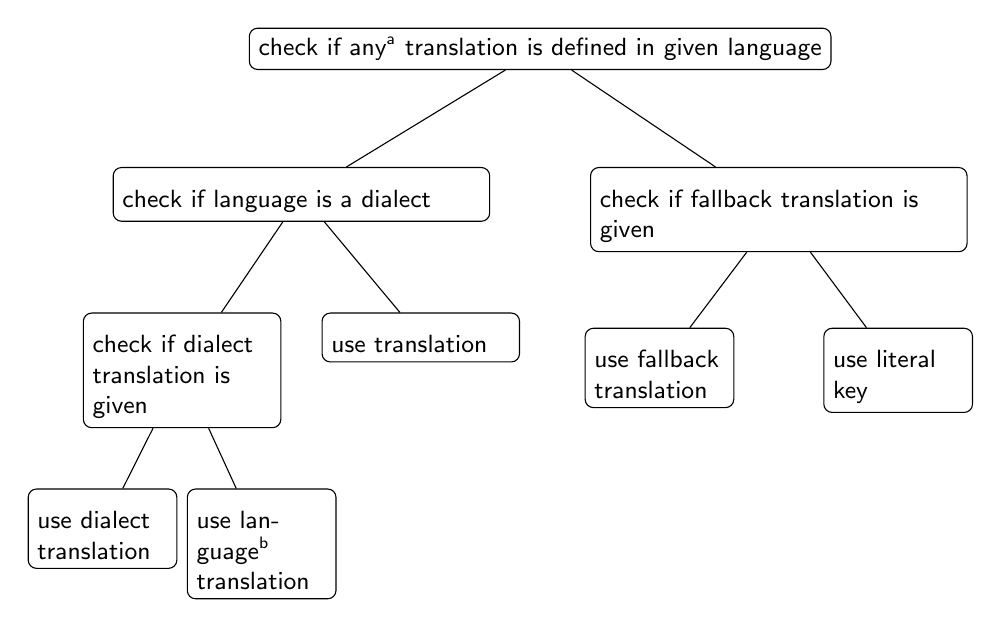
\begin{tikzpicture}
    [
      level/.style={sibling distance=.5\linewidth/#1},
      every node/.style={
        draw,
        rounded corners=3pt,
        align=left,
        anchor=north,
        font=\small\sffamily
      }
    ]
    \node {check if any\fnote{a}  translation is defined in given language}
      child {
        node[text width=\nodewidth]
          {\yes check if language is a dialect}
        child {
          node[text width=\nodewidth/2]
            {\yes check if dialect translation is given}
          child {
            node[text width=\nodewidth/2.75]
              {\yes use dialect translation}
          }
          child {
            node[text width=\nodewidth/2.75]
              {\no use lan\-guage\fnote{b} translation}
          }
        }
        child {
          node[text width=\nodewidth/2]
            {\no use translation}}
        }
      child {
        node[text width=\nodewidth]
          {\no check if fallback translation is given}
        child {
          node[text width=\nodewidth/2.75]
            {\yes use fallback translation}
        }
        child {
          node[text width=\nodewidth/2.75]
            {\no use literal key}
        }
      } ;
  \end{tikzpicture}
  \caption{Schematic representation of \translations' translating
    mechansim. Notes: \fnote{a} except for a possible fallback
    translation. \fnote{b} \ie, the base language of the dialect.}
  \label{fig:scheme}
\end{figure}

What happens if you declare a translation? There are four cases:
\begin{enumerate}
  \item You declare a translation for a base language: this is the normal case
    where an internal macro is defined which can be fetched by the
    \cs{GetTranslation} command (see \cref{ssec:commands}).
  \item You declare a translation for a language alias: this is the very same
    as the first case since the same internal macro is defined.
  \item You declare a translation for a dialect: this is two-fold.  Either a
    translation for the base language exists so only the translation for the
    dialect is saved.  If the translation for the base language does not exist
    it is defined to be the same as the one for the dialect.
  \item You declare a translation for an alias of a dialect: this is the very
    same as the third case as again the internal macros are the same.
\end{enumerate}

\subsection{Available Commands}\label{ssec:commands}
Below the commands provided by \translations\ are explained.  The symbol
\textcolor{expandable}{\expandablesign} means that the command is expandable.
Commands without the marker aren't expandable.

\begin{commands}
  \command{DeclareLanguage}[\marg{lang}]
    Declare a language that can be used by \translations.  If the language
    already exists it will be silently redefined.  This command can only be
    used in the preamble.  It should never be necessary to use this command as
    \translations\ already declares loads of languages (\cref{sec:languages}).
    Should you miss one please send me an email and I'll add it to
    \translations.
  \command{DeclareLanguageAlias}[\marg{lang2}\marg{lang1}]
    Declares \meta{lang2} to be an alias of \meta{lang1}.  If \meta{lang1}
    doesn't exist yet a warning will be raised and it will be defined.  This
    command can only be used in the preamble.  It should never be necessary to
    use this command as \translations\ already declares loads of languages
    (\cref{sec:languages}).  Should you miss one please send me an email and
    I'll add it to \translations.
  \command{DeclareLanguageDialect}[\marg{dialect}\marg{lang}]
    Declares \meta{dialect} to be a dialect of language \meta{lang}.  If a
    translation for \meta{dialect} is provided it is used by the translation
    macros.  If there is none the corresponding translation for \meta{lang}
    is used instead.  It should never be necessary to use this command as
    \translations\ already declares loads of languages (\cref{sec:languages}).
    Should you miss one please send me an email and I'll add it to
    \translations.
  \command{NewTranslation}[\marg{lang}\marg{key}\marg{translation}]
    Defines a translation of key \meta{key} for the language \meta{lang}.
    An error will be raised if a translation of \meta{key} already exists.
    This command can only be used in the preamble.
  \command{RenewTranslation}[\marg{lang}\marg{key}\marg{translation}]
    Redefines a translation of key \meta{key} for the language \meta{lang}.
    An error will be raised if no translation of \meta{key} exists.
    This command can only be used in the preamble.
  \command{ProvideTranslation}[\marg{lang}\marg{key}\marg{translation}]
    \sinceversion{1.2}Provides a translation of key \meta{key} for the
    language \meta{lang}. If a translation of \meta{key} already exists it
    won't be overwritten and no error will be raised.  This command can only
    be used in the preamble.
  \command{DeclareTranslation}[\marg{lang}\marg{key}\marg{translation}]
    Defines a translation of key \meta{key} for the language \meta{lang}.
    No error will be raised if a translation of \meta{key} already exists.
    This command can only be used in the preamble.
  \command{DeclareTranslationFallback}[\marg{key}\marg{fallback}]
    Defines a fallback translation for key \meta{key} that is used in case no
    translation of \meta{key} for the currently active language has been
    provided.  No error will be raised if a fallback for \meta{key} already
    exists.  This command can only be used in the preamble.
  \expandable\command{GetTranslationFor}[\marg{lang}\marg{key}]
    Fetches and prints the translation of \meta{key} for the language
    \meta{lang}.  This command is expandable.
  \expandable\command{GetTranslation}[\marg{key}]
    Fetches and prints the translation of \meta{key} for the currently active
    language (as for example set by \pkg{babel}).  This command is expandable.
  \expandable\command{GetLCTranslationFor}[\marg{lang}\marg{key}]
    \sinceversion{1.1}Fetches and prints the translation of \meta{key} for
    the language \meta{lang}.  This command ensures that the fetched
    translation is set lowercase.  This command is expandable (well, sort
    of: in an \cs*{edef} it leaves \cs*{lowercase}\marg{translation} in the
    input stream where \meta{translation} is what \cs{GetTranslationFor} would
    expand to).
  \expandable\command{GetLCTranslation}[\marg{key}]
    \sinceversion{1.1}Fetches and prints the translation of \meta{key} for
    the currently active language (as for example set by \pkg{babel}).  This
    command ensures that the fetched translation is set lowercase.  This
    command is expandable (well, sort of: in an \cs*{edef} it leaves
    \cs*{lowercase}\marg{translation} in the input stream where
    \meta{translation} is what \cs{GetTranslation} would expand to).
  \command{GetTranslationForWarn}[\marg{lang}\marg{key}]
    \sinceversion{1.0}Fetches and prints the translation of \meta{key} for
    the language \meta{lang}.  Issues a warning if no translation is
    available at the cost of expandability.
  \command{GetTranslationWarn}[\marg{key}]
    \sinceversion{1.0}Fetches and prints the translation of \meta{key} for
    the currently active language (as for example set by \pkg{babel}).
    Issues a warning if no translation is available at the cost of
    expandability.
  \command{GetLCTranslationForWarn}[\marg{lang}\marg{key}]
    \sinceversion{1.1}Fetches and prints the translation of \meta{key} for
    the language \meta{lang}.  This command ensures that the fetched
    translation is set lowercase.  Issues a warning if no translation is
    available at the cost of expandability.
  \command{GetLCTranslationWarn}[\marg{key}]
    \sinceversion{1.1}Fetches and prints the translation of \meta{key} for
    the currently active language (as for example set by \pkg{babel}).  This
    command ensures that the fetched translation is set lowercase.  Issues a
    warning if no translation is available at the cost of expandability.
  \command{SaveTranslationFor}[\marg{cmd}\marg{lang}\marg{key}]
    Fetches and saves the translation of \meta{key} for the language
    \meta{lang} in the macro \meta{cmd}.
  \command{SaveTranslation}[\marg{cmd}\marg{key}]
    Fetches and saves the translation of \meta{key} for the currently active
    language (as for example set by \pkg{babel}) in the macro \meta{cmd}.
  \command{LoadDictionary}[\marg{name}]
    Loads a file named \code{\meta{name}-\meta{lang}.trsl} where \meta{lang}
    corresponds to the lowercase name of the current language as defined with
    \cs{DeclareLanguage}.  This file should contain the translations for the
    specified language.
  \command{LoadDictionaryFor}[\marg{lang}\marg{name}]
    Loads a file named \code{\meta{name}-\meta{lang}.trsl}.
  \command{NewDictTranslation}[\marg{key}\marg{translation}]
    \sinceversion{0.10}This command is to be used in a dictionary file and
    picks up the language of that file.  Issues an error if either the
    translation for the \meta{key} or the dictionary entry for the \meta{key}
    already exists.
  \command{RenewDictTranslation}[\marg{key}\marg{translation}]
    \sinceversion{0.10}This command is to be used in a dictionary file and
    picks up the language of that file.  Issues an error if either the
    translation for the \meta{key} or the dictionary entry for the \meta{key}
    doesn't exist.
  \command{ProvideDictTranslation}[\marg{key}\marg{translation}]
    \sinceversion{0.10}This command is to be used in a dictionary file and
    picks up the language of that file.  Only defines the translation and adds
    a corresponding dictionary entry if they don't exist yet.  This command is
    used in the dictionaries that a part of \translations.
  \command{DeclareDictTranslation}[\marg{key}\marg{translation}]
    This command is to be used in a dictionary file and picks up the language
    of that file, see \cref{sec:dictionaries} for an example.  Defines the
    translation and adds a dictionary entry regardless if they exist or not.
  \command{ProvideDictionaryFor}[\marg{lang}\marg{name}\oarg{date}]
    Needs to be in a dictionary file.  This command tells \translations\ that
    the file indeed is a dictionary and also sets the language for the
    dictionary which is used by \cs{DeclareDictTranslation}.
  \expandable\command{PrintDictionaryFor}%
    [\marg{lang}\marg{name}\marg{pre}\marg{mid}\marg{post}]
    \sinceversion{1.0}Prints all entries of dictionary \meta{name} in
    language \meta{lang} in the order the entries have been declared.  For
    every entry the code\par
    \meta{pre}\meta{key}\meta{mid}\meta{translation}\meta{post}\par
    is printed.  The dictionary must have been loaded of course.  There is
    probably only a very limited number of use cases for this command.  (It
    was for example used to print \cref{tab:dict}.)
  \expandable\command{baselanguage}[\marg{lang}]
    \changedversion{1.2a}Returns the (internal) base name of the given language,
    language alias or language dialect.  For a dialect this expands to the
    name of language it is a dialect of.  For a base language (see
    section~\ref{ssec:languages:base}) this usually simply is the lowercase
    version of the name.\par
    \verbcode+\baselanguage{English}+ $\Rightarrow$ \code{english}\\
    \verbcode+\baselanguage{American}+ $\Rightarrow$ \code{english}
  \expandable\command{ifcurrentlanguage}[\marg{lang}\marg{true}\marg{false}]
    \sinceversion{1.2}Places \meta{true} in the input stream if the current
    language is \meta{lang}.  Note: a dialect counts as a language of it's own
    here.  \cs{ifcurrentlanguage}\Marg{English} will for example be
    \meta{false} if the current \pkg{babel} language is \code{american}.   
  \expandable\command{ifcurrentbaselanguage}[\marg{lang}\marg{true}\marg{false}]
    \sinceversion{1.2}Places \meta{true} in the input stream if the current
    language is \meta{lang}.  Note: a dialect does notcount as a language of
    it's own here.  If the current \pkg{babel} language is \code{american}
    then \cs{ifcurrentbaselanguage}\Marg{English} will be \meta{true}.
\end{commands}

\subsection{A Small Example}
This section demonstrates with two short examples how the macros are used.
The first example covers the basics: declaring of translations and then
retrieving and typesetting them.

\begin{example}
  % in the preamble:
  % \DeclareTranslation{English}{Kueche}{kitchen}
  % \DeclareTranslation{German}{Kueche}{K\"uche}
  % \DeclareTranslation{Spanish}{Kueche}{cocina}
  % \DeclareTranslation{French}{Kueche}{cuisine}
  
  \GetTranslation{Kueche}
  \SaveTranslation\kitchen{Kueche}
  \SaveTranslationFor\cuisine{french}{Kueche}

  \selectlanguage{ngerman}
  \GetTranslation{Kueche} \kitchen\ \GetTranslationFor{spanish}{Kueche}
  \cuisine
\end{example}

The next example demonstrates the use of dialects and how they fall back to
the translation for the main language if no extra translation was declared:

\begin{example}
  % in the preamble:
  % \DeclareTranslation{English}{farbe}{color}
  % \DeclareTranslation{British}{farbe}{colour}

  \GetTranslationFor{English}{farbe}
  \GetTranslationFor{British}{farbe}
  \GetTranslationFor{American}{farbe}
\end{example}

\subsection{Usage in Packages}
\subsubsection{Basic Structure}
A typical usage in a package would look as follows:
\begin{sourcecode}
  \RequirePackage{translations}
  \DeclareTranslationFallback{mypackage-title}{Nice Title}
  \DeclareTranslation{English}{mypackage-title}{Nice Title}
  \DeclareTranslation{French}{mypackage-title}{Beau Titre}
  \DeclareTranslation{German}{mypackage-title}{Sch\"{o}ner Titel} 
  ...
  \def\mypackage@title{\GetTranslation{mypackage-title}}
\end{sourcecode}

That is, a package defines some unique key for an expression and at least
defines a fallback translation.  Additionally translations for as many
languages as the author wants are defined.  A user then may add
\cs{DeclareTranslation}\marg{language}\marg{translation} if they find their
translation missing.

\subsubsection{The `fallback' language}
If a user has neither loaded \pkg{babel} nor \pkg{polyglossia} \translations\
will use English as language and translate to English if the translation was
provided.  If the user \emph{has} loaded one of the language packages but has
chosen a language for which no translation is defined the language `fallback'
will be used, \ie, the translation provided with
\cs{DeclareTranslationFallback}.  If no fallback translation is provided
either the translation will expand to the literal string.

The following three examples should make this concept clear:

\begin{example}[compile]
  \documentclass[margin=5mm]{standalone}
  \usepackage{translations}
  \DeclareTranslation{German}{foo-literal}{bar}
  \begin{document}
  \GetTranslation{foo-literal} % foo-literal
  \end{document}
\end{example}

\begin{example}[compile]
  \documentclass[margin=5mm]{standalone}
  \usepackage{translations}
  \DeclareTranslationFallback{foo-literal}{foo}
  \DeclareTranslation{German}{foo-literal}{bar}
  \begin{document}
  \GetTranslation{foo-literal} % foo
  \end{document}
\end{example}

\begin{example}[compile]
  \documentclass[margin=5mm]{standalone}
  \usepackage[ngerman]{babel}
  \usepackage{translations}
  \DeclareTranslation{German}{foo-literal}{bar}
  \begin{document}
  \GetTranslation{foo-literal} % bar
  \end{document}
\end{example}

\subsection{Dictionaries}\label{sec:dictionaries}
\subsubsection{Background}
\translations\ provides the means to write dictionary files that can be loaded
by packages or in a document.  Dictionaries can be loaded for the currently
active language with \cs{LoadDictionary} or for a specific language with
\cs{LoadDictionaryFor}. 

\begin{commands}
  \command{LoadDictionary}[\marg{name}]
    Loads a file named \code{\meta{name}-\meta{lang}.trsl} where \meta{lang}
    corresponds to the lowercase name of the current language as defined with
    \cs{DeclareLanguage}.  This file should contain the translations for the
    specified language.
  \command{LoadDictionaryFor}[\marg{lang}\marg{name}]
    Loads a file named \code{\meta{name}-\meta{lang}.trsl}.
\end{commands}

A package could provide dictionary files for its language dependent settings
and include the needed one at begin document.  The basics for creating a
dictionary file are explained in section~\ref{sec:own-dictionaries}.

\translations\ already provides a few basic dictionary files.  If the main
document language fits to one of the provided files the corresponding basic
dictionary is loaded at begin document by \translations, see
section~\ref{sec:transl-basic-dict} for more on this.

\subsubsection{Own Dictionaries}\label{sec:own-dictionaries}
A typical dictionary file should look as follows:
\begin{sourcecode}
  % this is file housing-german.trsl
  \ProvideDictionaryFor{German}{housing}[<version info>]
  \ProvideDictTranslation{kitchen (housing)}{K\"uche}
  \ProvideDictTranslation{bathroom (housing)}{Bad}
  \ProvideDictTranslation{living room (housing)}{Wohnzimmer}
  \ProvideDictTranslation{bedroom (housing)}{Schlafzimmer}
  ...
  \endinput
\end{sourcecode}

The usage is similar to the one in a package: unique keys are given
translations, this time for the language the dictionary file is declared for
only.  Translations can be declared by one of the following commands:
\begin{commands}
  \command{NewDictTranslation}[\marg{key}\marg{translation}]
    \sinceversion{0.10}This command is to be used in a dictionary file and
    picks up the language of that file.  Issues an error if either the
    translation for the \meta{key} or the dictionary entry for the \meta{key}
    already exists.
  \command{RenewDictTranslation}[\marg{key}\marg{translation}]
    \sinceversion{0.10}This command is to be used in a dictionary file and
    picks up the language of that file.  Issues an error if either the
    translation for the \meta{key} or the dictionary entry for the \meta{key}
    doesn't exist.
  \command{ProvideDictTranslation}[\marg{key}\marg{translation}]
    \sinceversion{0.10}This command is to be used in a dictionary file and
    picks up the language of that file.  Only defines the translation and adds
    a corresponding dictionary entry if they don't exist yet.  This command is
    used in the dictionaries that a part of \translations.
  \command{DeclareDictTranslation}[\marg{key}\marg{translation}]
    This command is to be used in a dictionary file and picks up the language
    of that file, see \cref{sec:dictionaries} for an example.  Defines the
    translation and adds a dictionary entry regardless if they exist or not.
\end{commands}

Every dictionary file \emph{must} contain the declaration
\cs{ProvideDictionaryFor}:
\begin{commands}
  \command{ProvideDictionaryFor}[\marg{lang}\marg{name}\oarg{date}]
    Needs to be in a dictionary file.  This command tells \translations\ that
    the file indeed is a dictionary and also sets the language for the
    dictionary which is used by \cs{NewDictTranslation} or similar commands.
\end{commands}

\subsubsection{\translations' Basic Dictionaries}\label{sec:transl-basic-dict}
\translations\ already provides a basic dictionary for the languages English,
French, German and Spanish.  This dictionary is loaded automatically if the
document language is one of these four.  If you'd like to contribute and add
the basic dictionary in your language this is more than welcome and highly
appreciated!  The easiest way to do this would be to copy one of the existing
files \code{translations-basic-dictionary-\meta{lang}.trsl} and modify the file
accordingly.  You can then send me the file via email and I'll add it to
\translations.

\Cref{tab:dict} lists all words provided by the basic dictionary for German.

\begin{longtable}{ll}
    \caption{All entries of \translations' basic dictionary in German.\label{tab:dict}} \\
    \toprule
    \rmfamily\bfseries key & \bfseries translation \\
    \midrule
  \endfirsthead
    \toprule
    \rmfamily\bfseries key & \bfseries translation \\
    \midrule
  \endhead
    \bottomrule
  \endlastfoot
    \midrule
    & \hfill\emph{continues} \\
  \endfoot
  \PrintDictionaryFor{German}{translations-basic-dictionary}{\ttfamily}{&}{\\}
\end{longtable}


\section{Defined Languages}\label{sec:languages}
\subsection{Base Languages}\label{ssec:languages:base}
Quite a number of languages already are defined, either directly or via an
alias.  So, before you define a language you should take a look at the tables
below if the language doesn't already exist.  \Cref{tab:languages} lists all
base languages, ``fallback'' being a dummy language used for fallback
translations.  \Cref{tab:languages,tab:dialects,tab:aliases} list \emph{all}
language names known to \translations.  However, they're not sorted
alphabetically but listed in the order they have been defined.  I tried to
make the definitions in an alphabetical order but sometimes rather grouped
related language names together.

If you miss a language or recognize a language that has falsely been declared
as an alias but should rather be a dialect or base language itself (or any
variation of this theme) please let me know, preferably with a short
explanation what's wrong and why.

\newcounter{column}
\gdef\seplang{%
  \stepcounter{column}%
  \ifnumless{\value{column}}{5}
    {&}
    {\\\setcounter{column}{0}}%
}
\def\do#1{#1\seplang}
\makeatletter
\begin{longtable}{lllll}
    \caption{Base languages defined by \translations, from left to right in
      the order of definition.\label{tab:languages}} \\
    \toprule
  \endfirsthead
    \toprule
  \endhead
    \bottomrule
  \endlastfoot
    \midrule
    &&&& \hfill\emph{continues} \\
  \endfoot
  \dolistloop\@trnslt@languages
\end{longtable}
\makeatother

\subsection{Language Dialects}\label{ssec:languages:dialects}
\translations\ also defines a few dialects of thebase languages.  They are
listed in \cref{tab:dialects}.  The decision what is a dialect and what is an
alias is not always clear.  I am no linguist so I looked up information
available on the internet.  A language that was described as
\enquote{standardized register} was always defined as a dialect.  For some
other languages it seemed to make sense, such as British or Austrian.  The
decisions are open for debate.

\setcounter{column}{0}
\gdef\seplang{%
  \ifnumgreater{\value{column}}{3}
    {\setcounter{column}{1}}
    {\stepcounter{column}}%
  \ifnumless{\value{column}}{4}
    {&}
    {\\}%
}
\def\aliases#1#2{#1\seplang #2\seplang}
\def\do#1{\aliases#1}
\makeatletter
\begin{longtable}{ll@{\hspace*{4em}}ll}
    \caption{All dialects defined by \translations, from left to right in the
      order of definition.\label{tab:dialects}}\\
    \toprule
     \bfseries dialect & \bfseries language &
     \bfseries dialect & \bfseries language \\
    \midrule
  \endfirsthead
    \toprule
     \bfseries dialect & \bfseries language &
     \bfseries dialect & \bfseries language \\
    \midrule
  \endhead
    \bottomrule
  \endlastfoot
    \midrule
    &&& \hfill\emph{continues} \\
  \endfoot
  \dolistloop\@trnslt@dialects@pair
\end{longtable}
\makeatother

\subsection{Language Aliases}\label{ssec:languages:aliases}
To most of the base languages and dialects at least one alias exists, the
uppercase variant.  This is due to the fact that it is common to write
language names uppercased.  For a number of languages aliases were defined in
order to match \pkg{babel}'s or \pkg{polyglossia}'s names for the
languages.  Others are defined because there apparently exist more than one
name for the same language.  The decisions are not consistent.  For example it
could be argued that \enquote{deutsch} is an alias of \enquote{German}.  I am
open to suggestions and improvements.  All defined aliases are listed in
\cref{tab:aliases}.

\setcounter{column}{0}
\makeatletter
\begin{longtable}{ll@{\hspace*{4em}}ll}
    \caption{All language aliases defined by \translations, from left to right
      in the order of definition.\label{tab:aliases}}\\
    \toprule
     \bfseries alias & \bfseries language &
     \bfseries alias & \bfseries language \\
    \midrule
  \endfirsthead
    \toprule
     \bfseries alias & \bfseries language &
     \bfseries alias & \bfseries language \\
    \midrule
  \endhead
    \bottomrule
  \endlastfoot
    \midrule
    &&& \hfill\emph{continues} \\
  \endfoot
  \dolistloop\@trnslt@aliases@pair
\end{longtable}
\makeatother

These languages \emph{should} cover all languages which are currently covered
by \pkg{babel} and \pkg{polyglossia} but very likely this is not the
case.  Should you miss a language please send me an email so I can add it to
\translations.

\section{Implementation}
\lstinputlisting[style=cnltx]{translations.sty}


\end{document}


